% !TeX spellcheck = pl_PL
\documentclass[]{article}
\usepackage{graphicx}
\usepackage[T1]{fontenc}
\usepackage[cp1250]{inputenc}
\usepackage{polski}
\usepackage{float}
\graphicspath{ {./res/} }
\usepackage[a4paper, total={6in, 8in}]{geometry}
%opening

\begin{document}


\begin{titlepage}


\date{11 Luty, 2020}
\title
{
\begin{center}
	
\includegraphics{logo}\\
	\Huge Pracownia Konfiguracji i Monta�u System�w Komutacyjnych\\		
	\Large \vspace{5mm} Sprawozdanie 2/Seria 2\\
	\large \smallskip Pomiary wybranych parametr�w traktu
	�wiat�owodowego za pomoc�
	reflektometru
	\pagenumbering{}
\end{center}
}
\author{\medskip Micha� Wili�ski, zesp� 3, grupa 2, klasa IIID}
\maketitle
\end{titlepage}
\pagenumbering{arabic}
\section{Cel �wiczenia}
Celem �wiczenia by�o nabycie umiej�tno�ci zwi�zanych z wykonywaniem pomiar�w �wiat�owodowych i obs�ug�
reflektometru �wiat�owodowego OTDR.
\section{Schemat pogl�dowy}
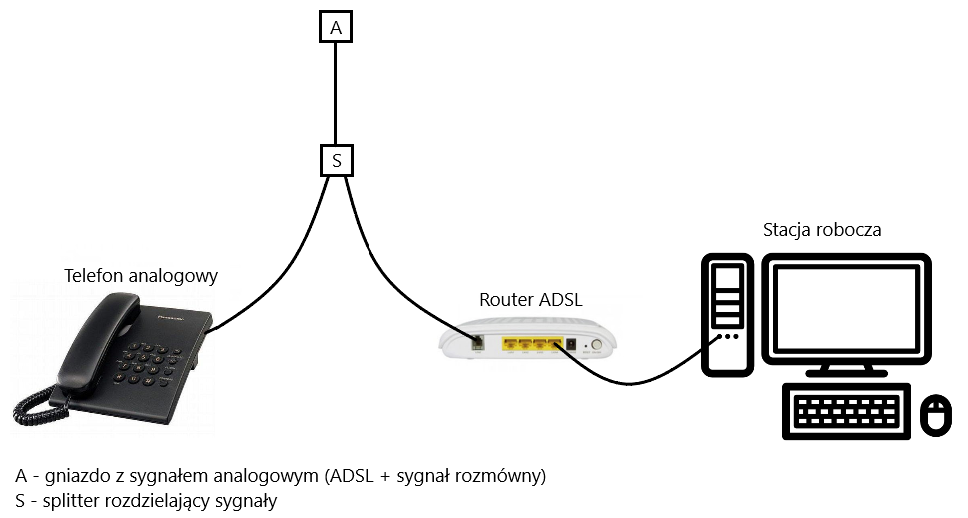
\includegraphics[scale=0.37]{schem}
\section{Wykonanie �wiczenia}
Na samym pocz�tku wykonali�my po��czenie jak na schemacie i ustawili�my parametry pomiaru takie jak \textbf{okno transmisyjne} (pierwszy pomiar odbywa� si� w II oknie - 1310nm) czy \textbf{szeroko�� impulsu sonduj�cego}. Spodziewana \textbf{d�ugo�� trasy} zosta�a ustawiona na 2km by pokaza� j� w ca�o�ci. Ustawili�my tak�e \textbf{rodzaj badanego �wiat�owodu} na jednomodowy i \textbf{metod� pomiaru t�umienia zdarze�} na LSA (metoda czteropunktowa).\\
\begin{figure}[H]
	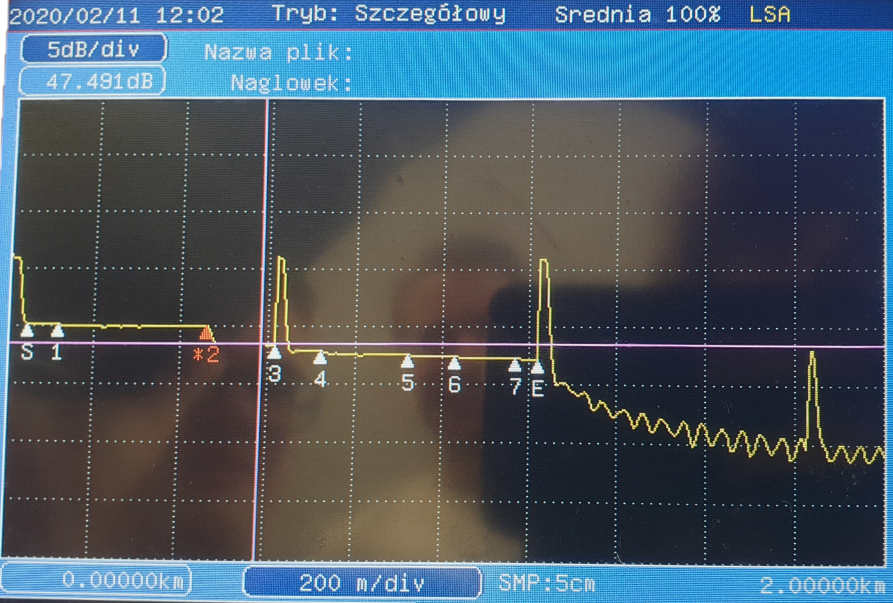
\includegraphics[width=100mm]{s1}
	\caption{Reflektogram pierwszej trasy w pierwszym kierunku }
	\label{fig:s1}
\end{figure}

\section{Wnioski}
\end{document}
